\documentclass{beamer}
\usepackage{graphicx}
\usepackage{booktabs}
\usepackage[most]{tcolorbox}
\usepackage{ragged2e}
\usepackage{amsmath, esint}
\usepackage[symbol]{footmisc}
\usepackage{tikz}
\usetikzlibrary{backgrounds, positioning, arrows, scopes, shapes, shapes.misc, shapes.multipart}
\tikzset{
    cross/.style={cross out, draw=black, minimum size=2*(#1-\pgflinewidth), inner sep=0pt, outer sep=0pt},
    cross/.default={10pt},
    split/.style={rectangle split, rectangle split parts=7, draw, inner sep=0ex, rectangle split horizontal, minimum size=4ex},
    textstyle/.style={text height=1.5ex, text depth=.25ex}
}

\usepackage{amsthm}
\usepackage{amstext}
\usepackage{amssymb}
%%\usepackage[plain]{algorithm}
%%\usepackage{algpseudocode}

\usepackage{minted}
\usepackage{xcolor} 
\definecolor{LightGray}{gray}{0.975}

%\usetheme{Warsaw}
\usefonttheme{serif} 

\title[L5 DP]{Introduction to Algorithms \\ Lecture 5: Dynamic Programming (DP)}
\author{Prof. Charles E. Leiserson and Prof. Erik Demaine \\ Massachusetts Institute of Technology}
\date{\today}

\setbeamertemplate{navigation symbols}{}%remove navigation symbols

\defbeamertemplate*{footline}{shadow theme}{%
    \leavevmode%
    \hbox{
        \begin{beamercolorbox}[wd=.5\paperwidth,ht=2.5ex,dp=1.125ex,leftskip=.3cm plus1fil,rightskip=.3cm]{author in head/foot}%
            \usebeamerfont{author in head/foot} Introduction to Algorithms: \hfill \insertshorttitle
        \end{beamercolorbox}%
        \begin{beamercolorbox}[wd=.5\paperwidth,ht=2.5ex,dp=1.125ex,leftskip=.3cm,rightskip=.3cm plus1fil]{title in head/foot}%
            \usebeamerfont{title in head/foot} \hfill \insertframenumber\,/\,\inserttotalframenumber%
        \end{beamercolorbox}
    }%
    \vskip0pt%
}

\AtBeginSection[]{
    \begin{frame}<beamer>
    \frametitle{Plan}
    \tableofcontents[currentsection]
    \end{frame}
}

\newcommand{\toRight}[1]{
    \begin{FlushRight}
        {\small #1}
    \end{FlushRight}
}

\begin{document}

\frame{\titlepage}

\begin{frame}{Introduction to Algorithms}
    \centering
    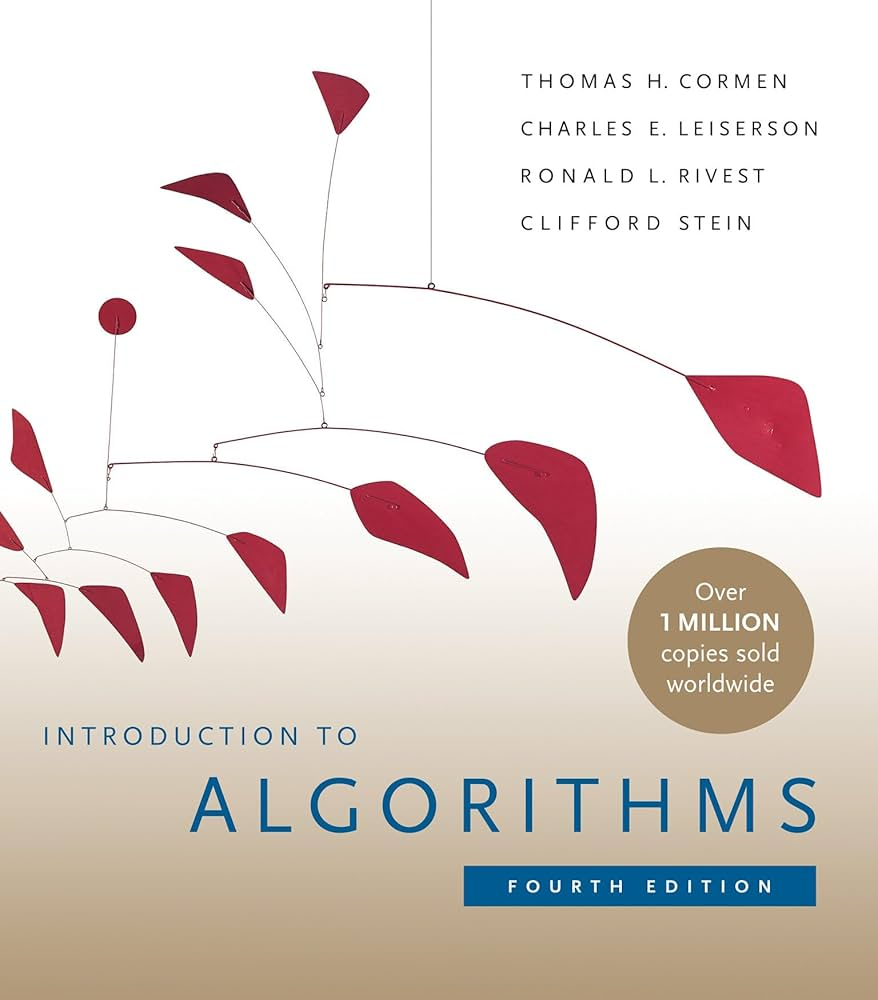
\includegraphics[width=0.45\textwidth]{figures/book_cover.jpg} \\
    \vspace{5mm}{
        \tiny
        Content has been extracted from \textit{Introduction to Algorithms}, Fourth Edition, by Cormen, Leiserson, Rivest, and Stein. MIT Press. 2022.\\
        Visit \url{https://mitpress.mit.edu/9780262046305/introduction-to-algorithms/}.\\
        Original slides from \textit{Introduction to Algorithms 6.046J/18.401J}, Fall 2005 Class by Prof. Charles Leiserson and Prof. Erik Demaine. MIT OpenCourseWare Initiative available at \url{https://ocw.mit.edu/courses/6-046j-introduction-to-algorithms-sma-5503-fall-2005/}.\\
    }
\end{frame}

\section{Dynamic Programming}

\begin{frame}{Dynamic Programming\footnote{\textit{Programming} in this context refers to a tabular method, not to writing computer code.} (DP)}
    \begin{itemize}
        \item Invented by Richard Bellman in 1950s.
        \item Desing technique, like Divide \& Conquer.
        \item Applies when the subproblems overlap --that is, when subproblems share subsubproblems.
        \item It solves each subsubproblem just once and then saves its answer in a table.
        \item DP typically applies to optimization problems:
        \begin{itemize}
            \item have many possible solutions.
            \item find a solution with the optimal (min or max) value.
            \item \textit{an} optimal solution, not \textit{the} optimal solution.
        \end{itemize}
    \end{itemize}
\end{frame}

\begin{frame}{DP notions}
    \begin{enumerate}
        \item Characterize the structure of an optimal solution.
        \item Recursively define the value of an optimal solution based on optimal solutions of subproblems.
        \item Compute the value of an optimal solution in bottom-up fashion (recursion \& memoization).
        \item Construct an optimal solution from the computed information.
    \end{enumerate}
    \vspace{10mm}
    \centering
    \Large
    \textcolor{blue}{\textbf{DP}} = \textcolor{orange}{\textbf{Recursion}} + \textcolor{olive}{\textbf{Memoization}}
\end{frame}

\begin{frame}{DP notions}
    \centering
    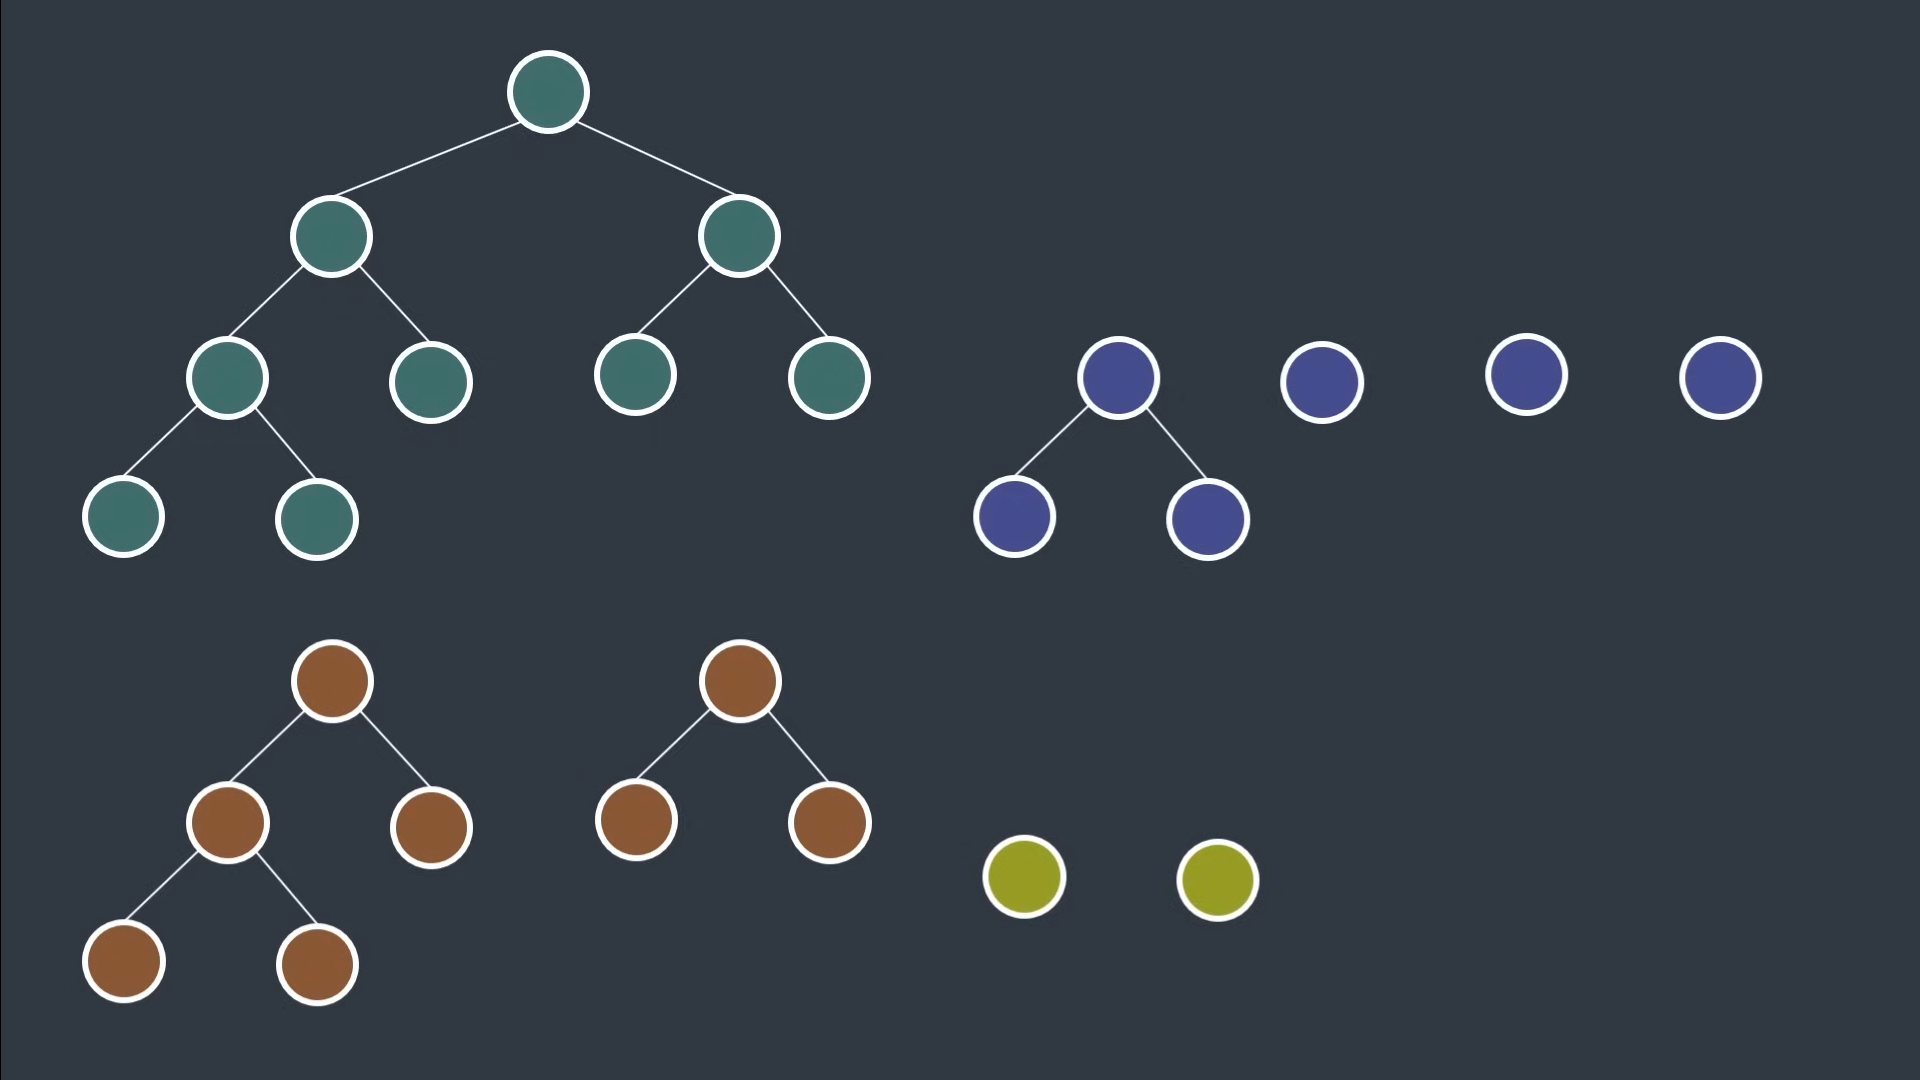
\includegraphics[width=\textwidth]{figures/dp01.png}
\end{frame}

\section{N-th Fibonacci Number}

\begin{frame}{N-th Fibonacci Number\footnote{\scriptsize \textit{Mastering Dynamic Programming - How to solve any interview problem (Part 1)}. Tech With Nikola Channel, 2024. YouTube, available at \url{https://youtu.be/Hdr64lKQ3e4?si=ycTe-hoyfaICRWXt}}}
    Write a function that returns the n-th Fibonacci number.
    \begin{equation*}
        \begin{align*}
            F_1 &= F_2 = 1 \\
            F_n &= F_{n - 1} + F_{n - 2} \\
        \end{align*}
    \end{equation*}
    \centering
    \LARGE
    \begin{tabular}{| c | c | c | c | c | c | c | c |} \hline
        n & 1 & 2 & 3 & 4 & 5 & 6 & 7  \\ \hline
    $F_n$ & 1 & 1 & 2 & 3 & 5 & 8 & 13 \\ \hline
    \end{tabular}
\end{frame}

\begin{frame}[fragile]{Naive Approach}
    \begin{minted}
    [tabsize=4, obeytabs, frame=lines, framesep=2mm, baselinestretch=1.2, bgcolor=LightGray, fontsize=\scriptsize, linenos]{python}
    def fib(n):
        if n <= 2:
            result = 1
        else:
            result = fib(n - 1) + fib(n - 2)
        return result
    \end{minted}
    \pause
    \begin{minted}
    [tabsize=4, obeytabs, framesep=2mm, baselinestretch=1.2, bgcolor=LightGray, fontsize=\scriptsize]{text}
    print(fib(7))
    Output: 13
    print(fib(50))
    Output: ???
    \end{minted}
\end{frame}

\begin{frame}{Naive Approach}
    \centering
    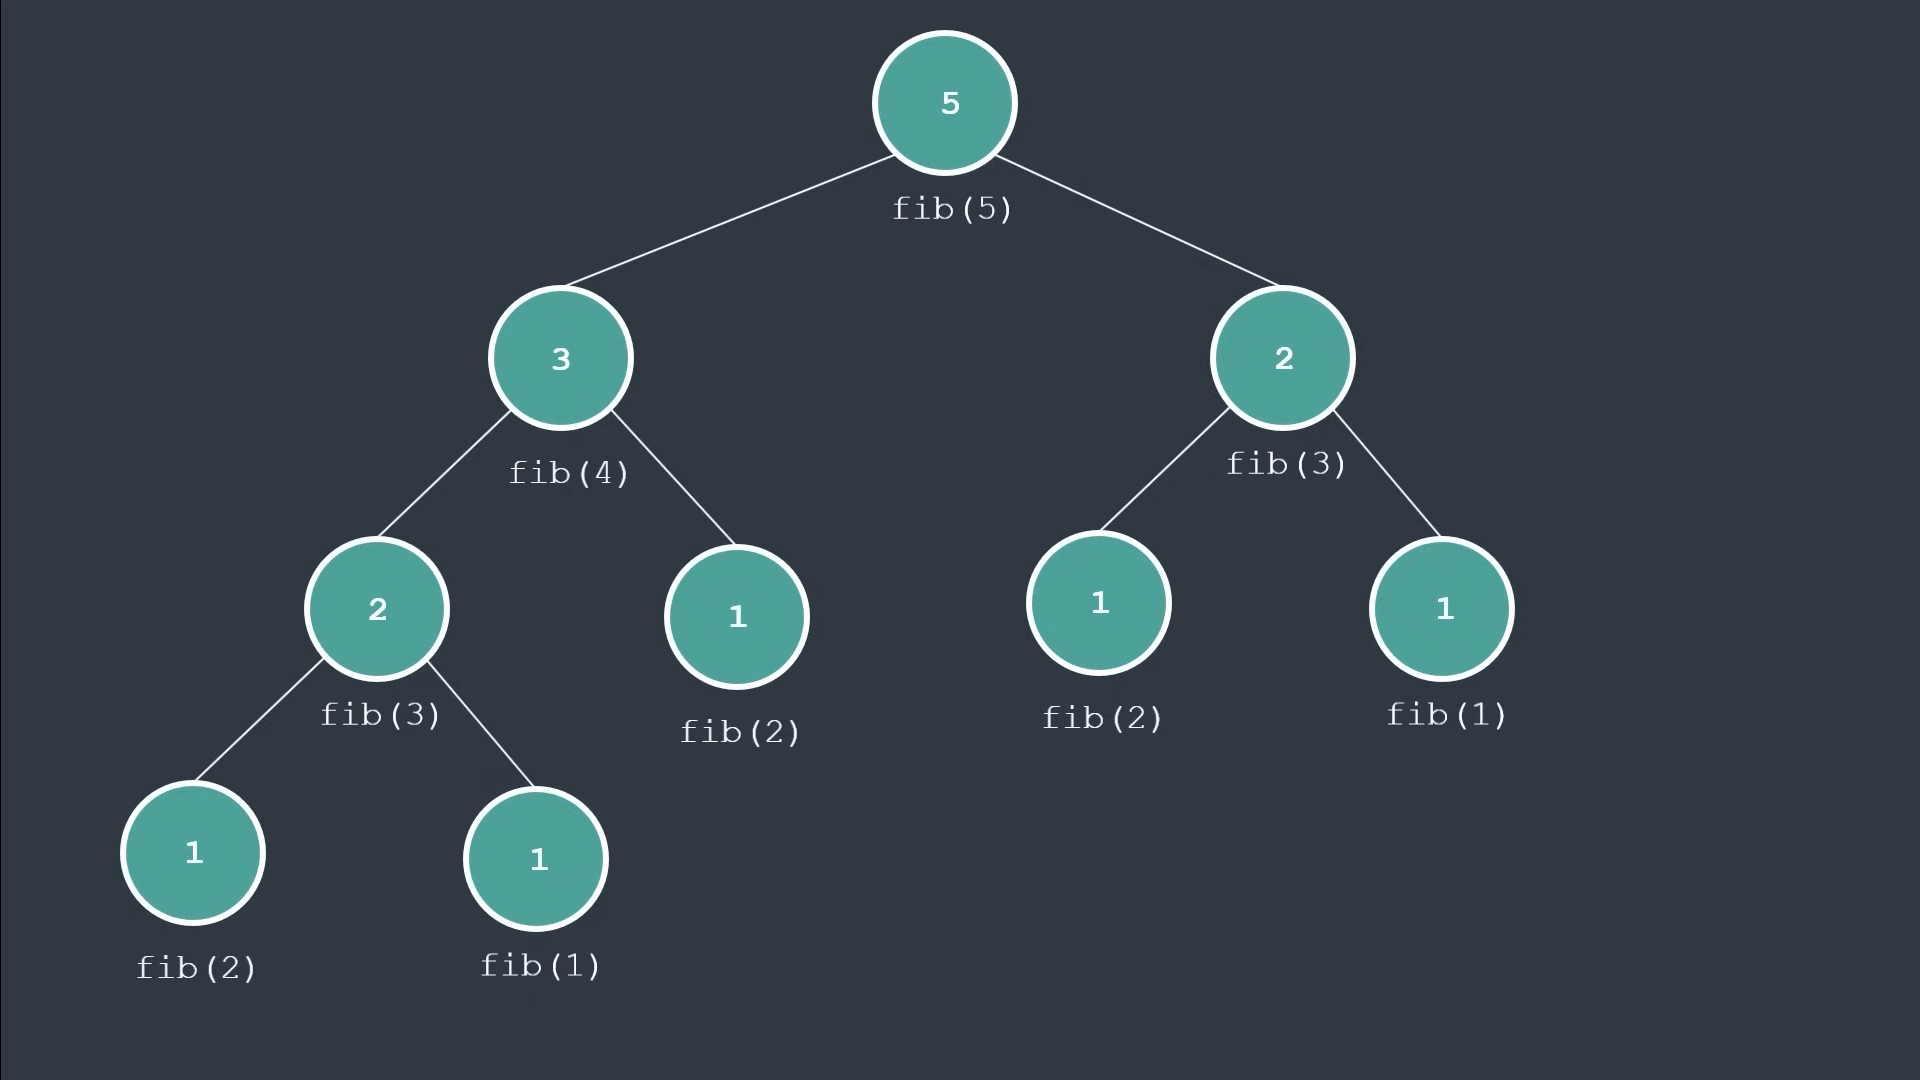
\includegraphics[width=\textwidth]{figures/fb01.png}
\end{frame}
\begin{frame}{Naive Approach}
    \centering
    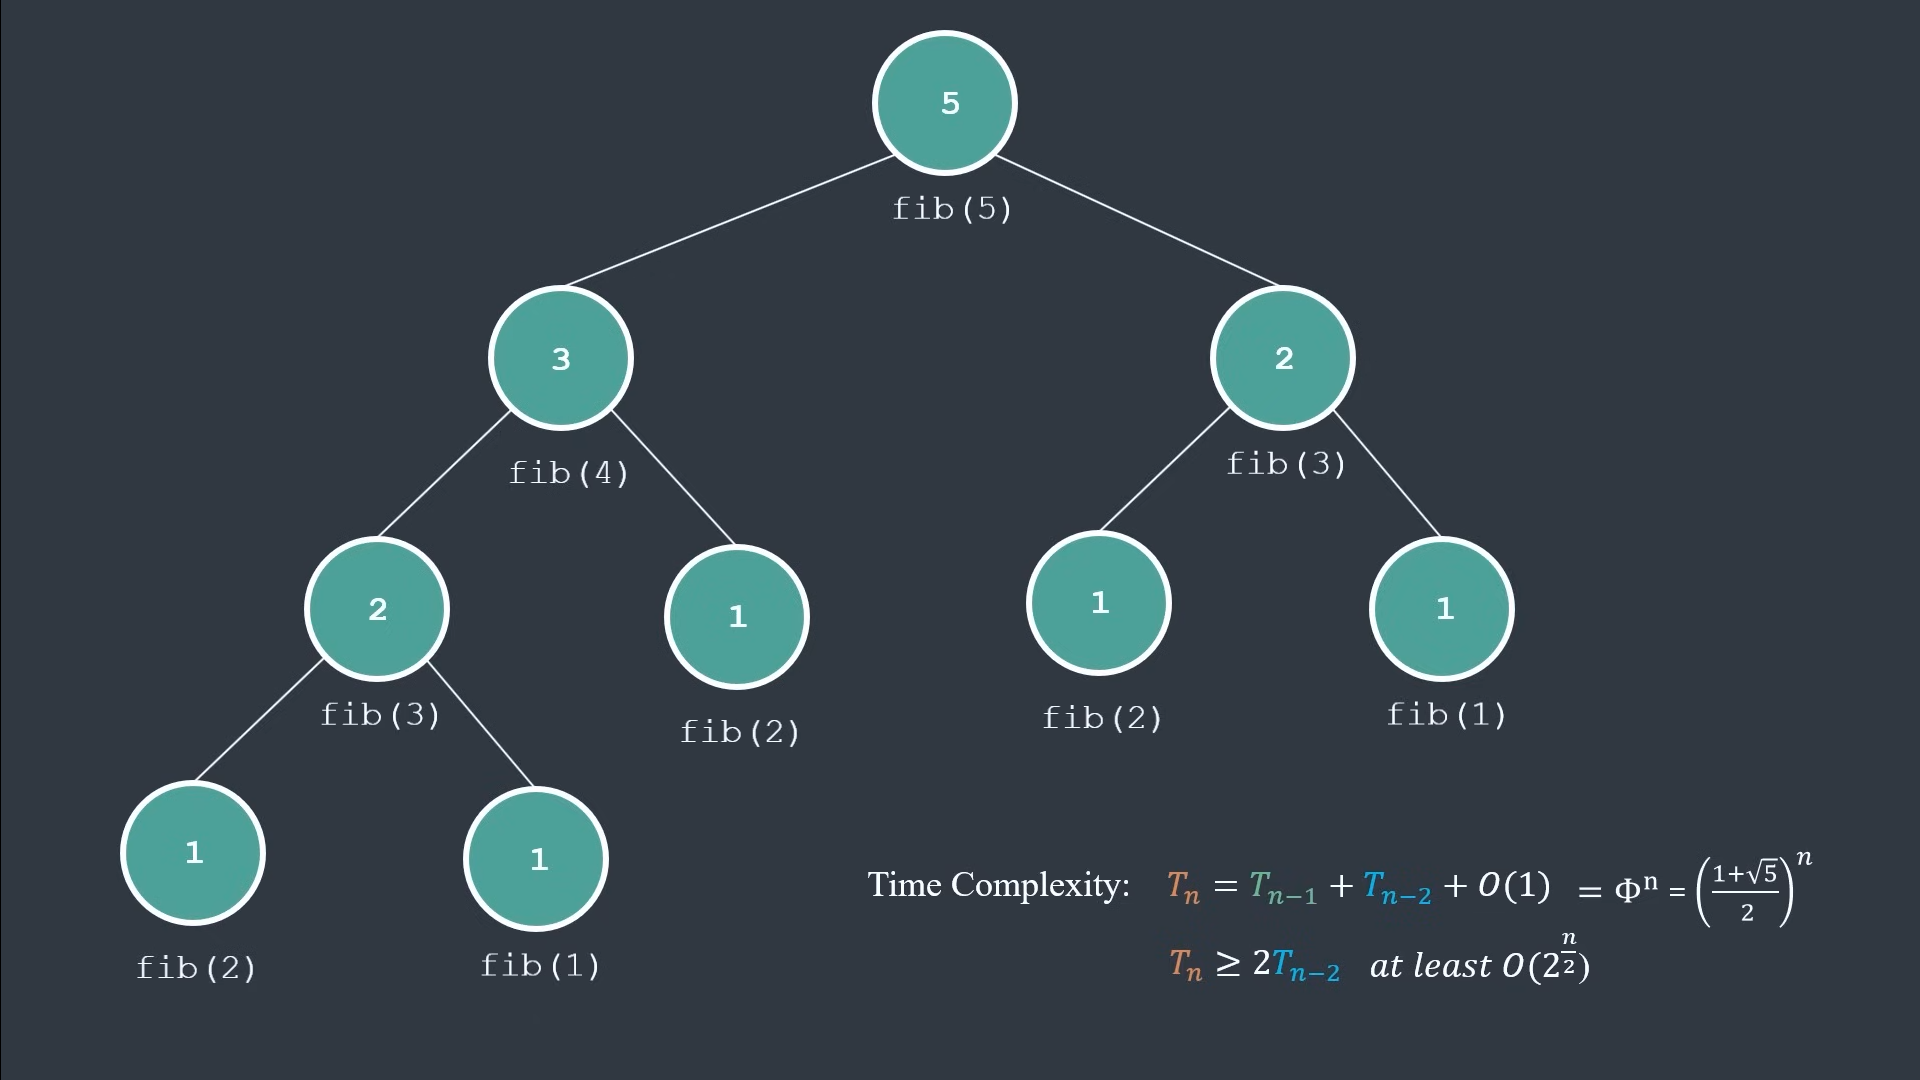
\includegraphics[width=\textwidth]{figures/fb02.png}
\end{frame}
\begin{frame}{Naive Approach}
    \centering
    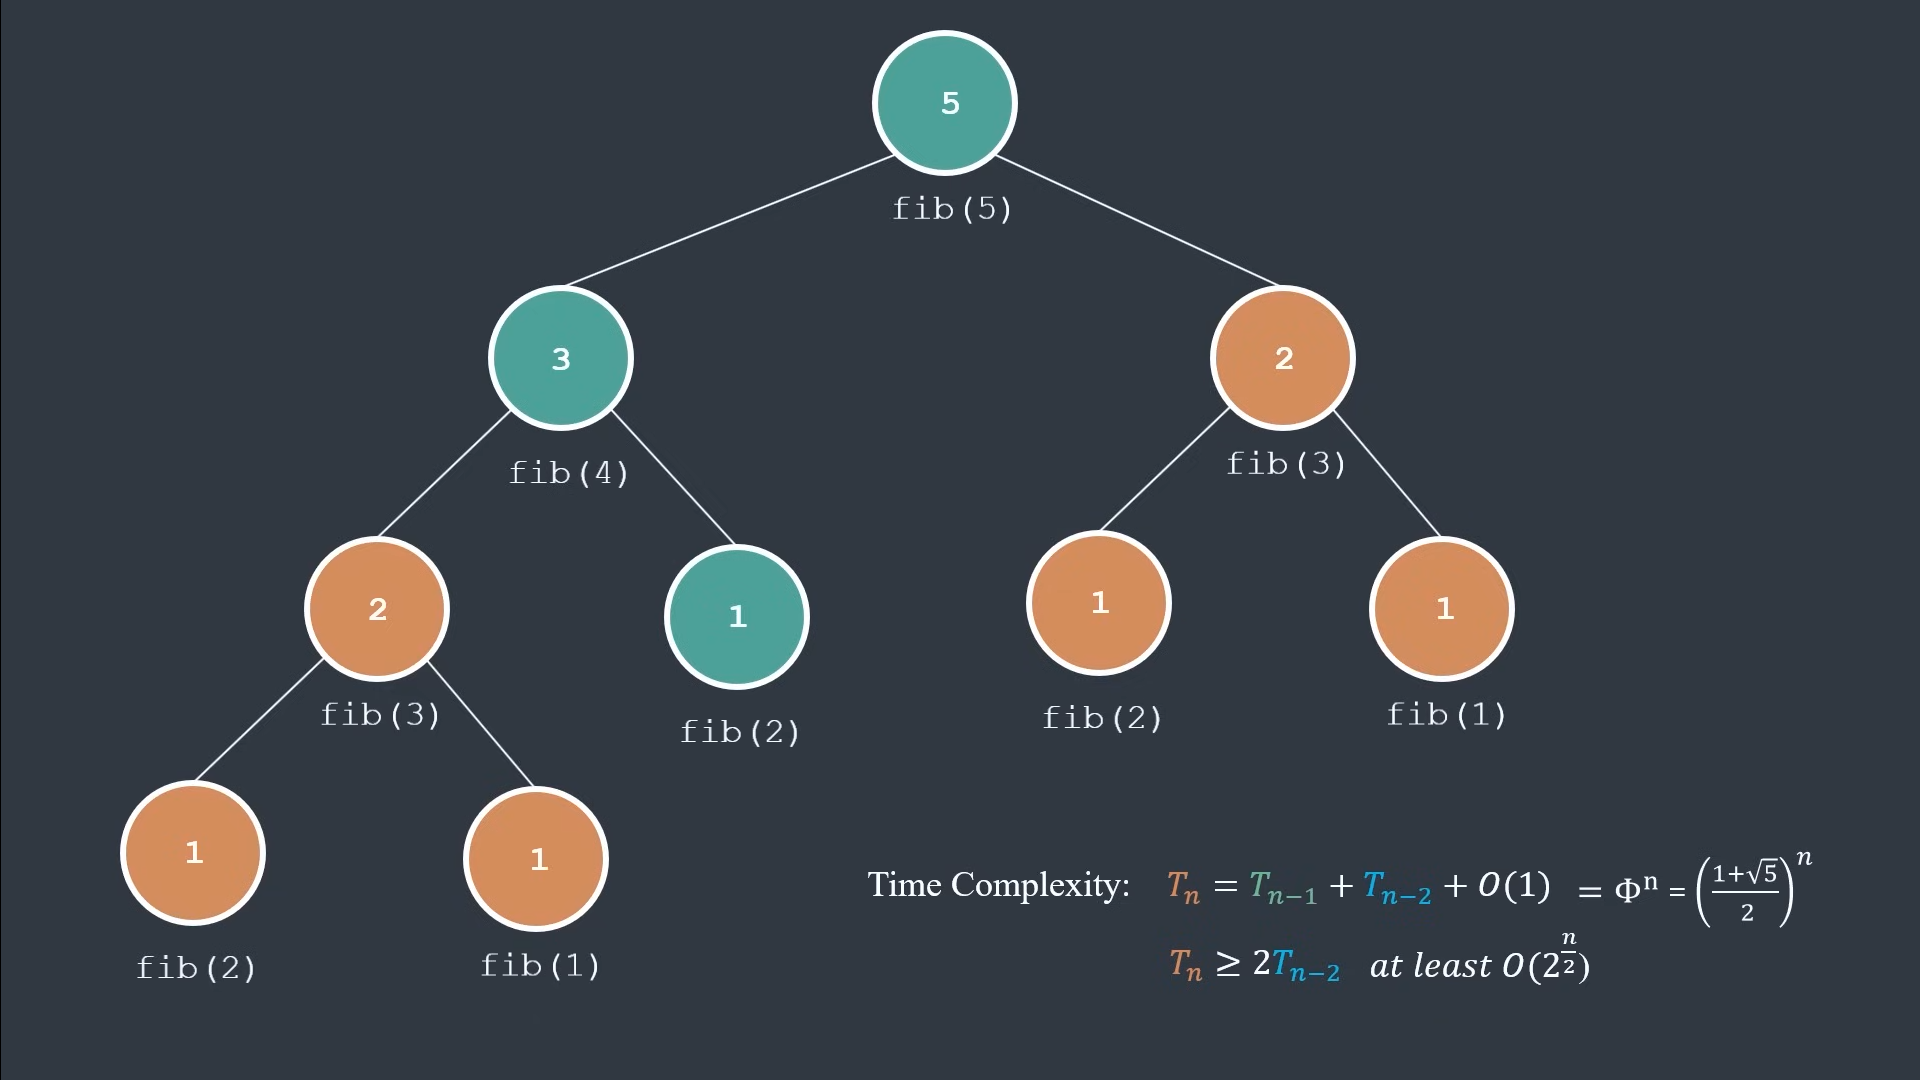
\includegraphics[width=\textwidth]{figures/fb03.png}
\end{frame}
\begin{frame}{Naive Approach}
    \centering
    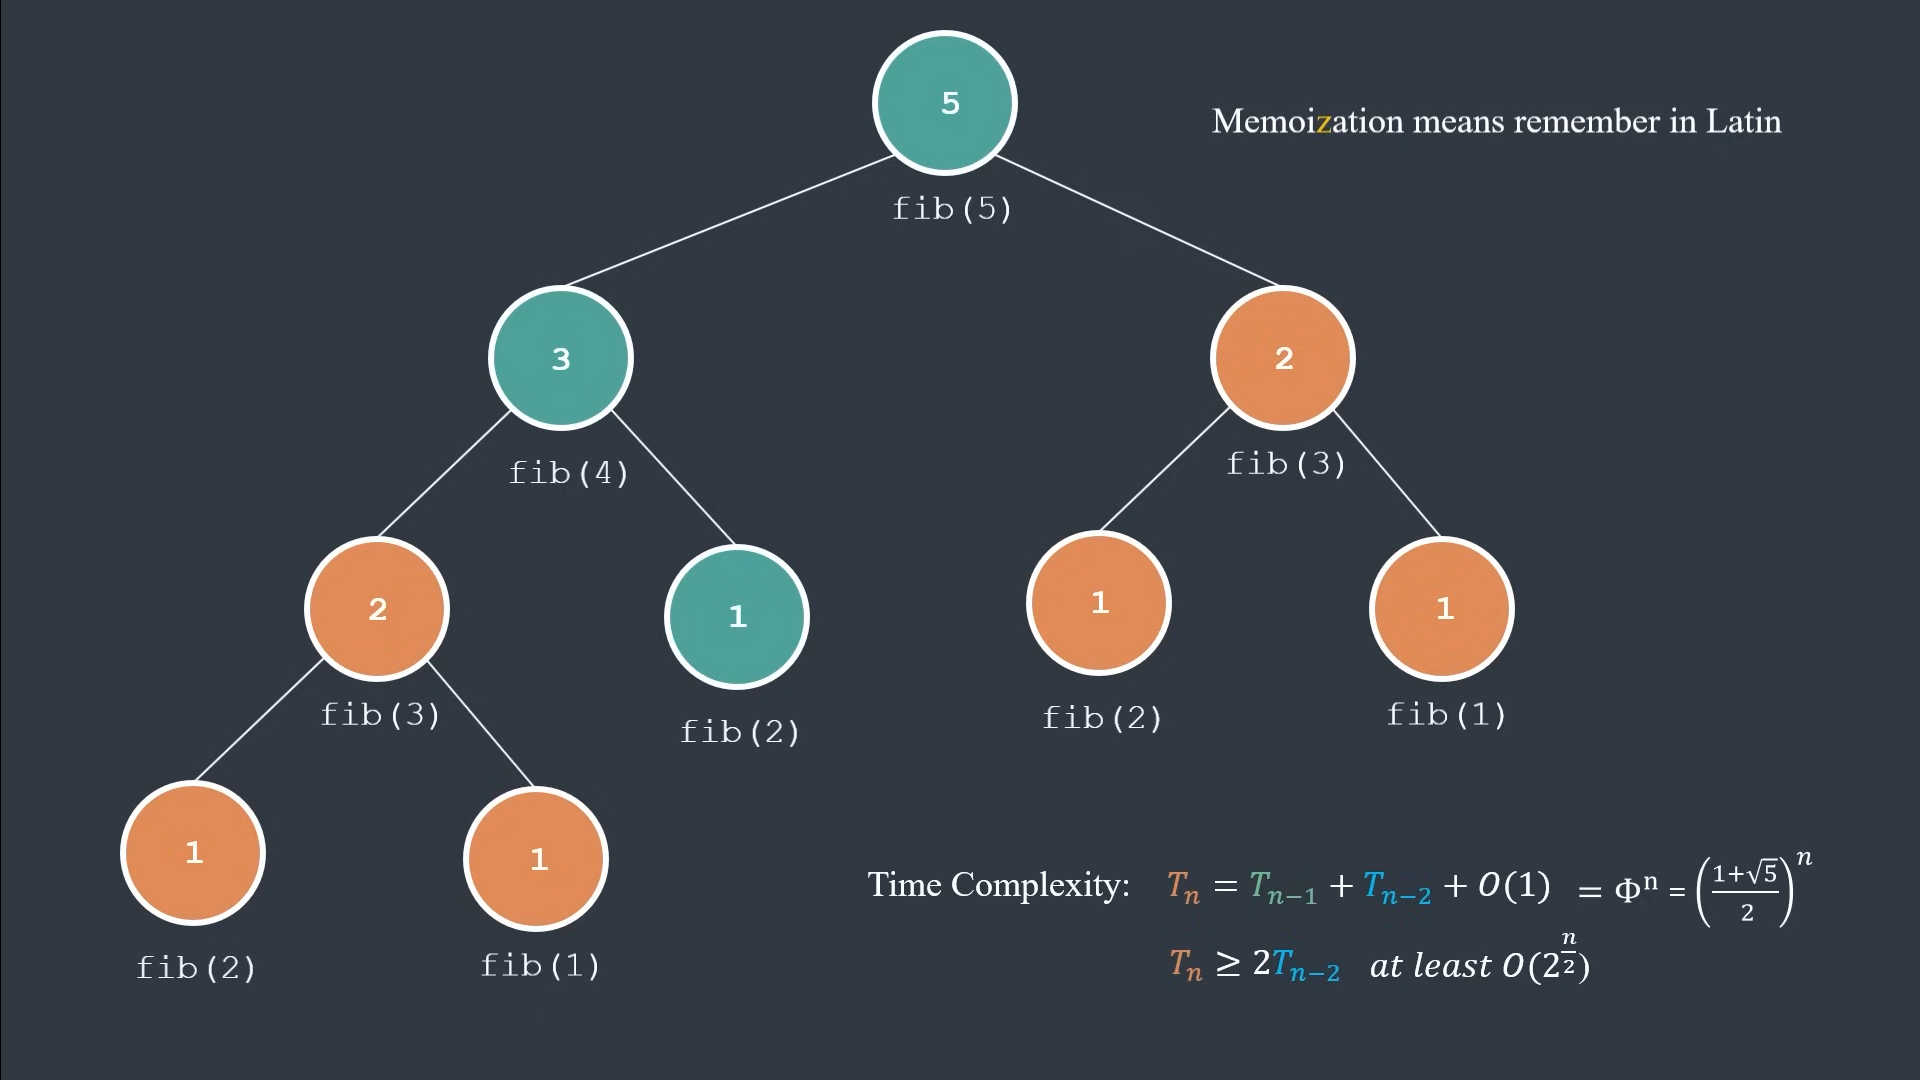
\includegraphics[width=\textwidth]{figures/fb04.png}
\end{frame}

\begin{frame}[fragile]{Memoization Approach}
    \begin{minted}
    [tabsize=4, obeytabs, frame=lines, framesep=2mm, baselinestretch=1.2, bgcolor=LightGray, fontsize=\scriptsize, linenos]{python}
    memo = {} # adding a dictionary...
    def fib(n):
        if n in memo: # asking if n is in dict...
            return memo[n] # if so, we are done!
        if n <= 2:
            result = 1
        else:
            result = fib(n - 1) + fib(n - 2)
        return result
    \end{minted}
    \pause
    \begin{minted}
    [tabsize=4, obeytabs, framesep=2mm, baselinestretch=1.2, bgcolor=LightGray, fontsize=\scriptsize]{text}
    print(fib(7))
    Output: 13
    print(fib(50))
    Output: 12586269025
    \end{minted}
    \pause
    \Large
    Time Complexity: $O(n)$.
\end{frame}

\begin{frame}{ }
    \centering
    \LARGE
    \textcolor{blue}{\textbf{DP}} = \textcolor{orange}{\textbf{Recursion}} + \textcolor{olive}{\textbf{Memoization}}
\end{frame}

\begin{frame}[fragile]{Bottom-up Approach}
    \begin{minted}
    [tabsize=4, obeytabs, frame=lines, framesep=2mm, baselinestretch=1.2, bgcolor=LightGray, fontsize=\scriptsize, linenos]{python}
    def fib(n):
        memo = {}
        for i in range(1, n + 1):
            if i <= 2:
                result = 1
            else:
                result = memo[n - 1] + memo[n - 2]
            memo[i] = result
        return memo[n]
    \end{minted}
\end{frame}

\begin{frame}{ }
    \centering
    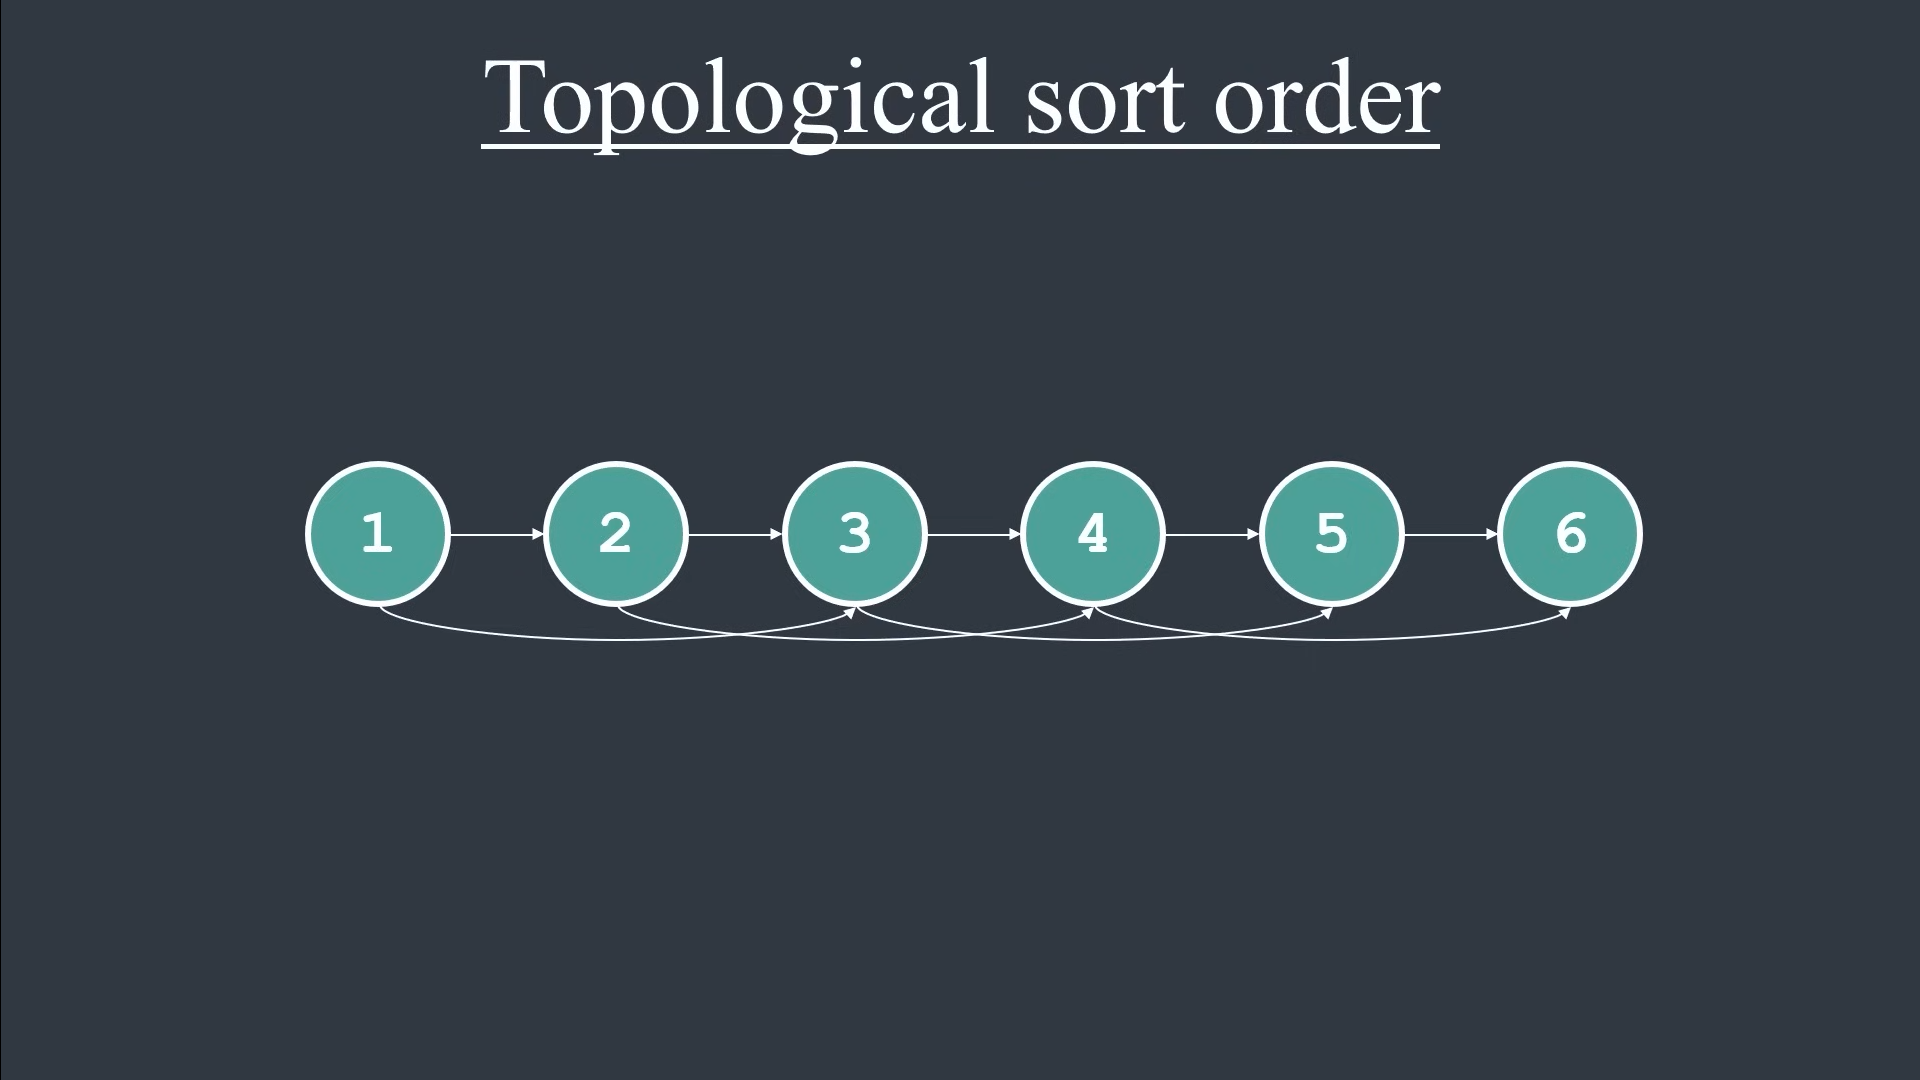
\includegraphics[width=\textwidth]{figures/topo.png}
\end{frame}

\section{Longest Palindromic Sequence}

\begin{frame}{Longest Palindromic Sequence}
    \begin{exampleblock}{Definition:}
        A palindrome is a string that is unchanged when reversed.
    \end{exampleblock}
    \begin{itemize}
     \item Examples: \texttt{radar}, \texttt{civic}, \texttt{t}, \texttt{bb}, \texttt{redder}.
     \item Given: A string $X[1 \ldots n]$, $n \geq 1$.
     \item To find: Longest palindrome that is a subsequence.
     \item Example: Given ``c h a r a c t e r''.
     \item Output: ``c a r a c''.
     \item Answer will be $\geq 1$ in length.
    \end{itemize}
\end{frame}

\begin{frame}[fragile]{Strategy}
    $L(i, j)$: length of longest palindromic subsequence of $X[i \ldots j]$ for $i \leq j$.
    \begin{minted}
    [tabsize=4, obeytabs, frame=lines, framesep=2mm, baselinestretch=1.2, bgcolor=LightGray, fontsize=\scriptsize, linenos]{python}
    def L(i, j):
        if i == j:
            return 1
        if X[i] == X[j]:
            if i + 1 == j:
                return 2
            else:
                return 2 + L(i + i, j - 1)
        else:
            return max( L(i + 1, j), L(i, j - 1) )
    \end{minted}
\end{frame}

\begin{frame}{Analysis}
    As written, program can run in exponential time: suppose all symbols $X[i]$ are distinct.
    \begin{equation*}
        \begin{align*}
            T(n) &= \text{running time on input of length } n \\
            T(n) &=
                    \begin{cases}
                        1         & n = 1 \\
                        2T(n - 1) & n > 1 \\
                    \end{cases} \\
                 &= 2^{n - 1}
        \end{align*}
    \end{equation*}
\end{frame}

\begin{frame}{What is missing?}
    \begin{itemize}
        \item Complexity is exponential... why? \pause
        \item We are still not completing all the DP notions...
        \item There is \textbf{recursion} but there is not \textbf{Memoization}... \pause
        \item Cache is missing!
        \item There is a single line of code that will fix it...
    \end{itemize}
\end{frame}

\begin{frame}{Understanding the Subproblems}
    The problem typically involves checking whether a substring of a given string is a palindrome. If the input string has a length of \( n \), then the natural way to define subproblems is:
    \begin{itemize}
        \item Consider all possible substrings $s[i:j]$ of the string.
        \item For each substring, determine whether it is a palindrome.
    \end{itemize}
\end{frame}

\begin{frame}{Counting the Subproblems}
    A substring is defined by two indices, \( i \) (starting index) and \( j \) (ending index), where \( 0 \leq i \leq j < n \). This means:
    \begin{itemize}
        \item \( i \) can take values from \( 0 \) to \( n-1 \).
        \item For each \( i \), \( j \) can take values from \( i \) to \( n-1 \).
    \end{itemize}
\end{frame}

\begin{frame}{Total Number of Subproblems}
    The total number of such \( (i, j) \) pairs (i.e., total subproblems) is given by the summation:
    \[
    \sum_{i=0}^{n-1} (n - i) = n + (n-1) + (n-2) + \dots + 1
    \]
    Using the formula for the sum of the first \( n \) natural numbers:
    \[
    \sum_{k=1}^{n} k = \frac{n(n+1)}{2}
    \]
    Thus, the number of subproblems is:
    \[
    n^2
    \]
\end{frame}

\begin{frame}{Formula for Computing the Complexity of a DP}
    \begin{large}
        \texttt{\# of subproblems} $\times$ \texttt{time to solve each subproblem}
    \end{large}
    \toRight{Given that smaller ones are already solved\footnote{lookup is $\Theta(1)$}.}
    \bigskip
    So,
    \begin{itemize}
        \item Given $n^2$ distinct subproblems...
        \item By solving each subproblem only once...
        \item Running time reduces to:
            {\LARGE
            $$
                \Theta(n^2) \cdot \Theta(1) = \Theta(n^2)
            $$
            }
    \end{itemize}
\end{frame}

\begin{frame}[fragile]{New Strategy}
    \begin{itemize}
        \item Memoize $L(i, j)$, hash inputs to get output value, and lookup hash table to see if the subproblem is already solved, else recurse.
    \end{itemize}

    \begin{minted}
    [tabsize=4, obeytabs, frame=lines, framesep=2mm, baselinestretch=1.2, bgcolor=LightGray, fontsize=\scriptsize, linenos]{python}
    def L(i, j):
        if i == j:
            return 1
        if X[i] == X[j]:
            if i + 1 == j:
                return 2
            else:
                return 2 + L(i + i, j - 1)
        else:
            return max( L(i + 1, j), L(i, j - 1) )
    \end{minted}
    \pause
    \begin{tikzpicture}[remember picture, overlay, node distance=3cm, text width=4cm, on grid, auto]
        \draw[orange, very thick, ->](5.35, 4.00) to [out=180,in=0](2.40, 4.575);
        \draw (7.50, 4.00) node[draw, orange, very thick, text=black]
            {\scriptsize
                Look at \verb|L[i, j]|
                and don't recurse if
                \verb|L[i, j]| is already
                computed.
            };
    \end{tikzpicture}
\end{frame}

\begin{frame}{Memoizing Vs. Iterating}
    \begin{enumerate}
        \item Memoizing uses a dictionary for $L(i, j)$ where value of $L$ is looked up by using $i, j$ as a key. Could just use a 2-D array here where null entries signify that the problem has not yet been solved.
        \item Can solve subproblems in order of increasing $j - i$ so smaller ones are solved first.
    \end{enumerate}
\end{frame}

\section{Longest Common Subsequence}

\begin{frame}{}
    \begin{itemize}
        \item Given two sequences $x[1 \cdots m]$ and $y[1 \cdots n]$, find a\footnote[2]{``a'' not ``the''} longest subsequence common to them both.
    \end{itemize} \pause
    \vspace{10mm}
    {\Huge x: \texttt{A B C B D A B}}\\
    \\
    {\Huge y: \texttt{B D C A B A}} \\
    \begin{itemize} \pause
        \item BDA ? \pause
        \item BDAB \pause
        \item BCAB \pause
        \item BCBA \pause
    \end{itemize}
    \texttt{LCS(x, y)} as notation not function...
\end{frame}

\begin{frame}{Brute-force LCS algorithm}
    \begin{itemize} \pause
        \item Check every subsequence of $x[1 \cdots m]$ to see if it is also a subsequence of $y[1 \cdots n]$.
    \end{itemize} \pause
    \begin{exampleblock}{Analysis}
        \begin{itemize}
            \item Checking = $O(n)$ time per subsequence.
            \item $2^m$ subsequences of $x$ (each bit-vector of length $m$ determines a distinct subsequence of $x$).
        \end{itemize}
        Worst-case running time $= O(n2^m)$ \pause \textcolor{red}{\textbf{Exponential time!}}
    \end{exampleblock}
\end{frame}

\begin{frame}{Towards a Better Algorithm}
    \begin{exampleblock}{Simplification:}
        \begin{enumerate}
            \item Look at the \textcolor{red}{\textit{length}} of a longest-common subsequence.
            \item Extend the algorithm to find the LCS itself.
        \end{enumerate}
    \end{exampleblock}
    \begin{itemize} \pause
        \item \textcolor{red}{\textbf{Notation:}} Denote the length of a sequence $s$ as $|s|$. \pause
        \item \textcolor{red}{\textbf{Strategy:}} Consider \textbf{prefixes} of $x$ and $y$:
            \begin{itemize}
                \item Define $c[i, j] = | LCS(x[1 \cdots i], y[1 \cdots j]) |$.
                \item Then, $c[m, n] = | LCS(x, y) |$.
            \end{itemize}
    \end{itemize}
\end{frame}

\begin{frame}{Recursive formulation}
    \begin{tcolorbox}[title=Theorem]
        \begin{equation*}
            \begin{align*}
                c[i, j] &=
                            \begin{cases}
                                0 & \text{ if } i = 0 \text{ or } j = 0 \text{, } \\
                                c[i - 1, j - 1] & \text{ if } x[i] = y[j] \text{, } \\
                                \max \{ c[i, j - 1], c[i - 1, j] \} & \text{ otherwise.}
                            \end{cases}
            \end{align*}
        \end{equation*}
    \end{tcolorbox}
    \textcolor{red}{\textbf{Proof:}} Case $x[i] = y[j] \ldots$ \\
    \\
    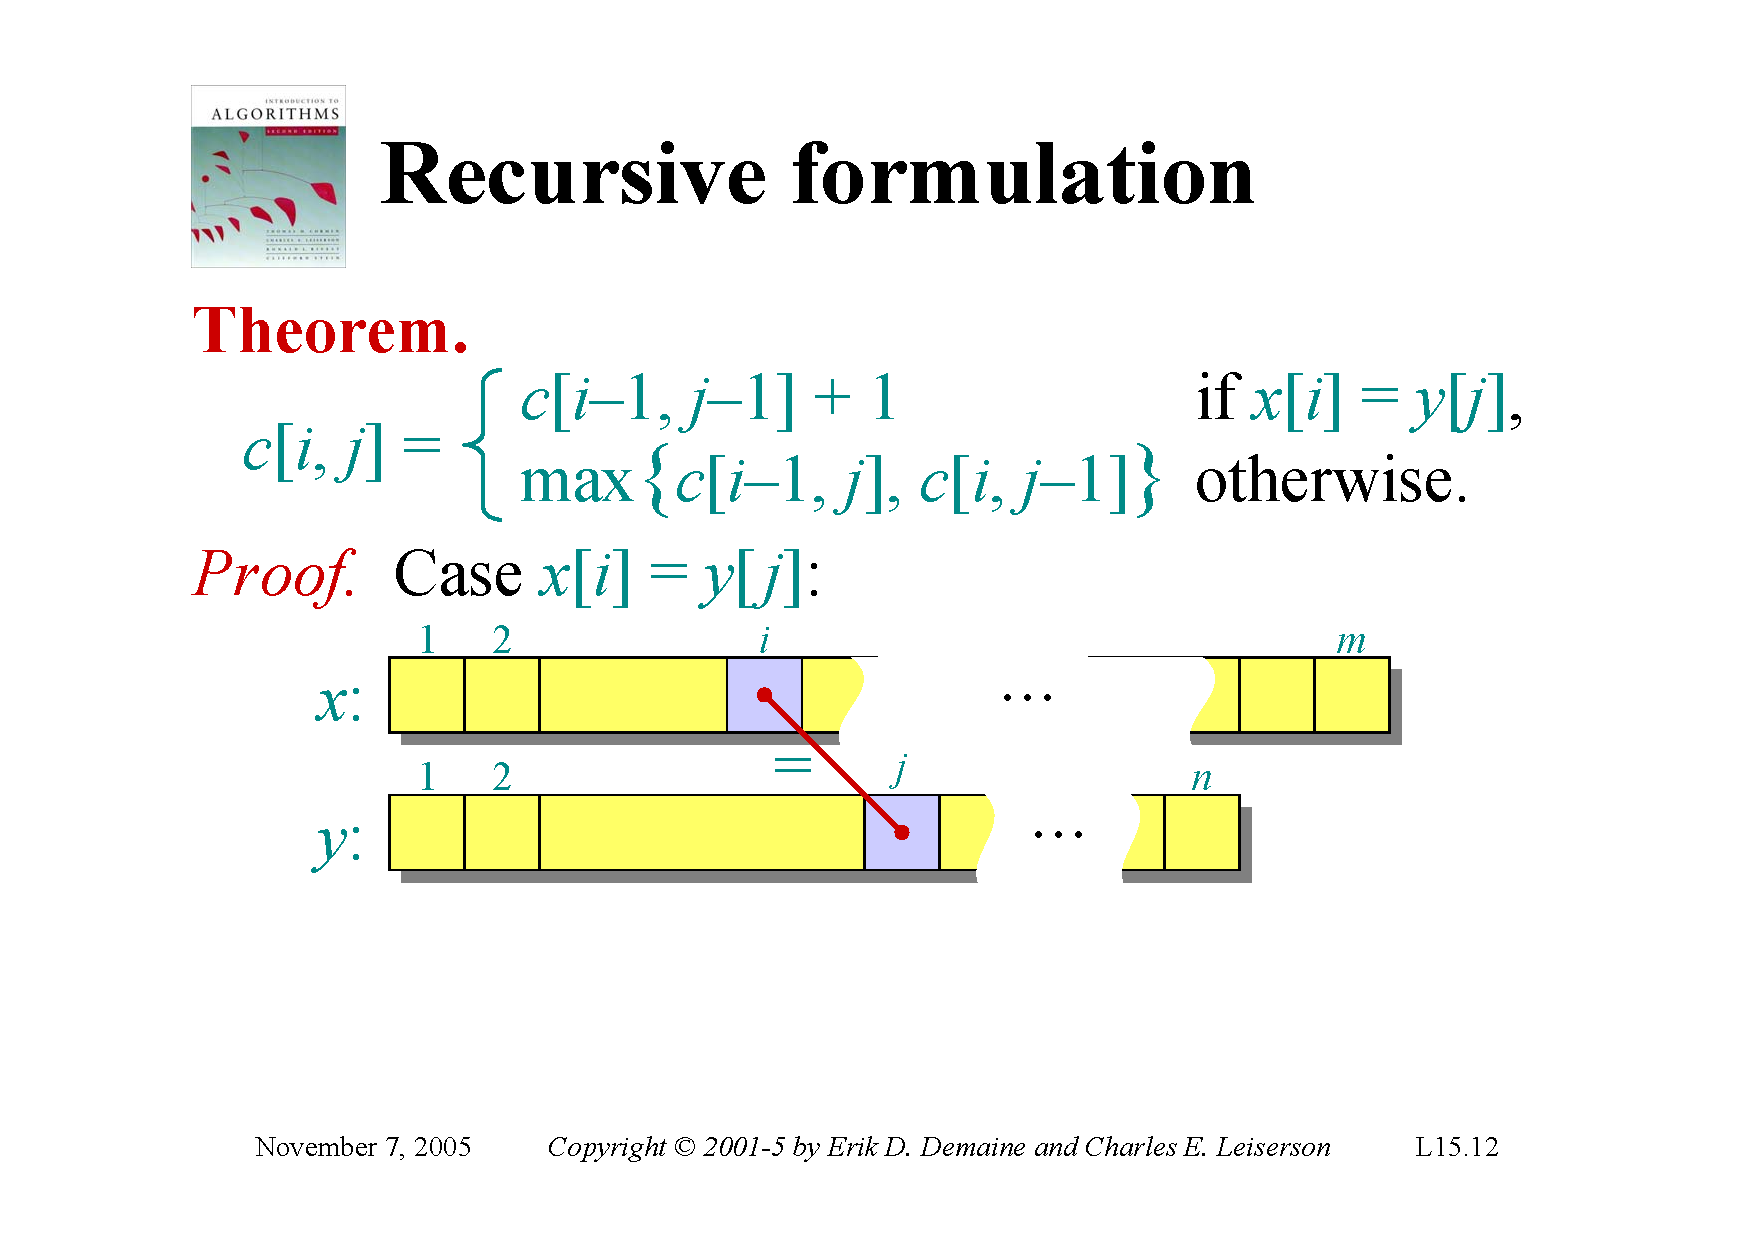
\includegraphics[width=\textwidth,trim=3cm 5cm 3cm 10.50cm, clip]{figures/proof01.pdf}
\end{frame}

\begin{frame}{Recursive formulation}
    \textcolor{red}{\textbf{Proof:}} Case $x[i] = y[j] \ldots$ \\
    \\
    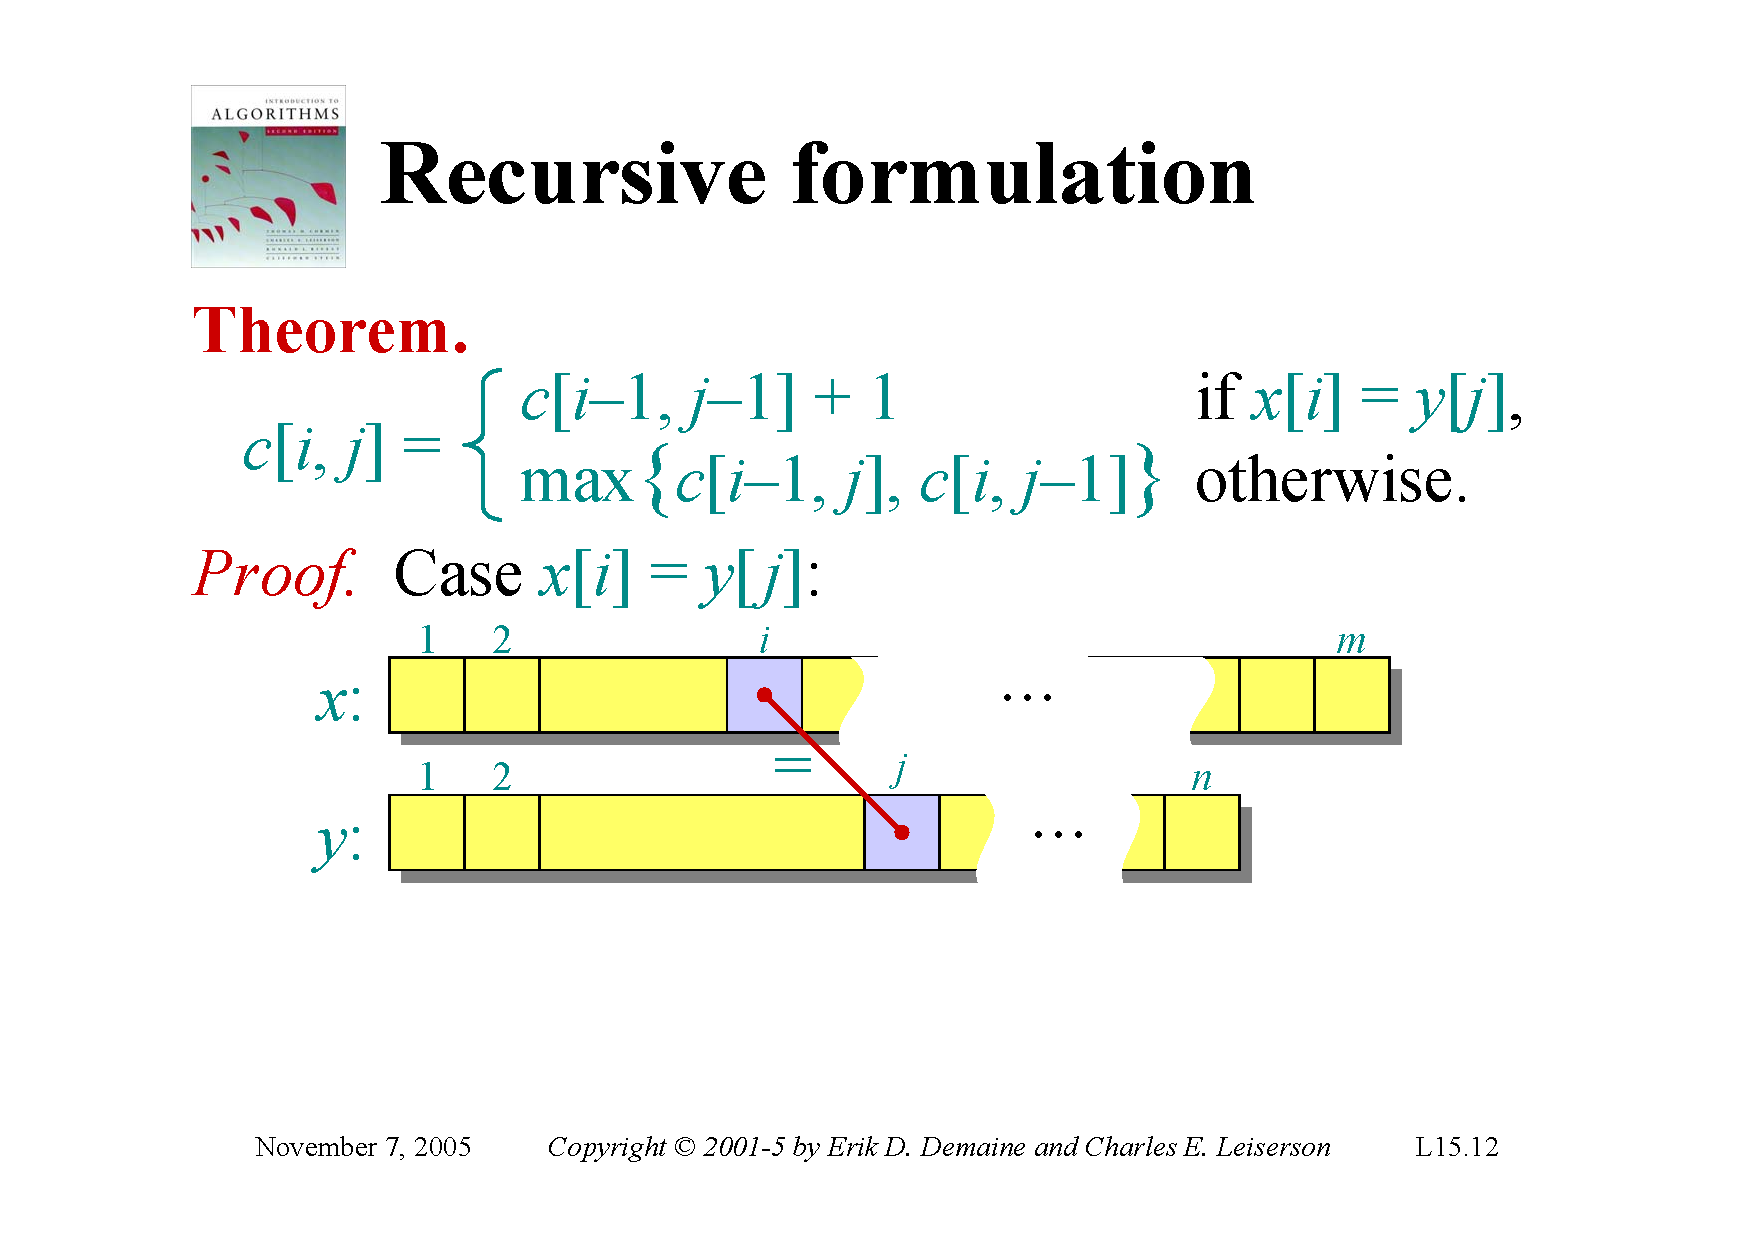
\includegraphics[width=\textwidth,trim=3cm 5cm 3cm 10.50cm, clip]{figures/proof01.pdf}
    \begin{itemize}
        \item Let $z[1 \cdots k] = LCS(x[1 \cdots i], y[1 \cdots j])$, where $c[i, j] = k$. \pause
        \item Then, $z[k] =$ \pause $x[i] ( = y[j])$\pause, or else $z$ could be extended. \pause
        \item Thus, $z[1 \cdots k–1]$ is CS of $x[1 \cdots i - 1]$ and $y[1 \cdots j - 1]$.
    \end{itemize}
\end{frame}

\begin{frame}{Step-by-Step Example of LCS Algorithm}
    We will use the dynamic programming (DP) approach to compute the LCS for the following strings:\\

    {\Huge X = ``ACDBE''} \\
    \\
    {\Huge Y = ``ABCDE''}
\end{frame}

\begin{frame}{Step 1: Create a DP Table}
    \begin{itemize}
        \item We construct a $(m+1) \times (n+1)$ table, where $m$ and $n$ are the lengths of $X$ and $Y$, respectively. The table will store the LCS length at each step.
        \item \textbf{Initial Table (before computation):} We initialize the first row and first column with 0s (LCS of empty strings is 0).
    \end{itemize}
\end{frame}

\begin{frame}{Step 1: Create a DP Table}
    \centering
    \begin{tabular}{|c|c|c|c|c|c|c|} \hline
                      & $\varnothing$ & A & B & C & D & E \\ \hline
        $\varnothing$ &        0      & 0 & 0 & 0 & 0 & 0 \\ \hline
               A      &        0      &   &   &   &   &   \\ \hline
               C      &        0      &   &   &   &   &   \\ \hline
               D      &        0      &   &   &   &   &   \\ \hline
               B      &        0      &   &   &   &   &   \\ \hline
               E      &        0      &   &   &   &   &   \\ \hline
    \end{tabular}
\end{frame}

\begin{frame}{Step 2: Fill the DP Table Using Recurrence}
    We iterate over each character of $X$ and $Y$ and apply the recurrence:
    \begin{equation*}
        \begin{align*}
            L[i, j] &=
                        \begin{cases}
                            L[i - 1, j - 1] + 1 & \text{ if } x[i] = y[j] \text{, } \\
                            \max \{ c[i, j - 1], c[i - 1, j] \} & \text{ otherwise.}
                        \end{cases}
        \end{align*}
    \end{equation*}
    \centering
    \begin{tabular}{|c|c|c|c|c|c|c|} \hline
                      & $\varnothing$ & A & B & C & D & E \\ \hline
        $\varnothing$ &        0      & 0 & 0 & 0 & 0 & 0 \\ \hline
               A      &        0      &   &   &   &   &   \\ \hline
               C      &        0      &   &   &   &   &   \\ \hline
               D      &        0      &   &   &   &   &   \\ \hline
               B      &        0      &   &   &   &   &   \\ \hline
               E      &        0      &   &   &   &   &   \\ \hline
    \end{tabular}
\end{frame}

\begin{frame}{Step 2: Fill the DP Table Using Recurrence}{Filling the table...}
    \vspace{-10mm}
    \scriptsize
    \begin{equation*}
        \begin{align*}
            L[i, j] &=
                        \begin{cases}
                            L[i - 1, j - 1] + 1 & \text{ if } x[i] = y[j] \text{, } \\
                            \max \{ c[i, j - 1], c[i - 1, j] \} & \text{ otherwise.}
                        \end{cases}
        \end{align*}
    \end{equation*}
    \begin{itemize}
        \item Compare `A' ($X[1]$) with each character in $Y$.
        \item `A' matches `A' $\longrightarrow L[1,1] = L[0,0] + 1 = 1$.
        \item Other cells get the max of left or top.
    \end{itemize}
    \vspace{6mm}
    \normalsize
    \centering
    \begin{tabular}{|c|c|c|c|c|c|c|} \hline
                      & $\varnothing$ & A & B & C & D & E \\ \hline
        $\varnothing$ &        0      & 0 & 0 & 0 & 0 & 0 \\ \hline
               A      &        0      & 1 & 1 & 1 & 1 & 1 \\ \hline
               C      &        0      &   &   &   &   &   \\ \hline
               D      &        0      &   &   &   &   &   \\ \hline
               B      &        0      &   &   &   &   &   \\ \hline
               E      &        0      &   &   &   &   &   \\ \hline
    \end{tabular}
\end{frame}

\begin{frame}{Step 2: Fill the DP Table Using Recurrence}{Filling the table...}
    \vspace{-10mm}
    \scriptsize
    \begin{equation*}
        \begin{align*}
            L[i, j] &=
                        \begin{cases}
                            L[i - 1, j - 1] + 1 & \text{ if } x[i] = y[j] \text{, } \\
                            \max \{ c[i, j - 1], c[i - 1, j] \} & \text{ otherwise.}
                        \end{cases}
        \end{align*}
    \end{equation*}
    \begin{itemize}
        \item Compare `C' ($X[2]$) with each character in $Y$.
        \item `C' matches `C' $\longrightarrow L[2,3] = L[1,2] + 1 = 2$.
        \item Other cells get the max of left or top.
    \end{itemize}
    \vspace{6mm}
    \normalsize
    \centering
    \begin{tabular}{|c|c|c|c|c|c|c|} \hline
                      & $\varnothing$ & A & B & C & D & E \\ \hline
        $\varnothing$ &        0      & 0 & 0 & 0 & 0 & 0 \\ \hline
               A      &        0      & 1 & 1 & 1 & 1 & 1 \\ \hline
               C      &        0      & 1 & 1 & 2 & 2 & 2 \\ \hline
               D      &        0      &   &   &   &   &   \\ \hline
               B      &        0      &   &   &   &   &   \\ \hline
               E      &        0      &   &   &   &   &   \\ \hline
    \end{tabular}
\end{frame}

\begin{frame}{Step 2: Fill the DP Table Using Recurrence}{Filling the table...}
    \vspace{-10mm}
    \scriptsize
    \begin{equation*}
        \begin{align*}
            L[i, j] &=
                        \begin{cases}
                            L[i - 1, j - 1] + 1 & \text{ if } x[i] = y[j] \text{, } \\
                            \max \{ c[i, j - 1], c[i - 1, j] \} & \text{ otherwise.}
                        \end{cases}
        \end{align*}
    \end{equation*}
    \begin{itemize}
        \item Compare `D' ($X[3]$) with each character in $Y$.
        \item `D' matches `D' $\longrightarrow L[3,4] = L[2,3] + 1 = 3$.
        \item Other cells get the max of left or top.
    \end{itemize}
    \vspace{6mm}
    \normalsize
    \centering
    \begin{tabular}{|c|c|c|c|c|c|c|} \hline
                      & $\varnothing$ & A & B & C & D & E \\ \hline
        $\varnothing$ &        0      & 0 & 0 & 0 & 0 & 0 \\ \hline
               A      &        0      & 1 & 1 & 1 & 1 & 1 \\ \hline
               C      &        0      & 1 & 1 & 2 & 2 & 2 \\ \hline
               D      &        0      & 1 & 1 & 2 & 3 & 3 \\ \hline
               B      &        0      &   &   &   &   &   \\ \hline
               E      &        0      &   &   &   &   &   \\ \hline
    \end{tabular}
\end{frame}

\begin{frame}{Step 2: Fill the DP Table Using Recurrence}{Filling the table...}
    \vspace{-10mm}
    \scriptsize
    \begin{equation*}
        \begin{align*}
            L[i, j] &=
                        \begin{cases}
                            L[i - 1, j - 1] + 1 & \text{ if } x[i] = y[j] \text{, } \\
                            \max \{ c[i, j - 1], c[i - 1, j] \} & \text{ otherwise.}
                        \end{cases}
        \end{align*}
    \end{equation*}
    \begin{itemize}
        \item Compare `B' ($X[4]$) with each character in $Y$.
        \item `B' matches `B' $\longrightarrow L[4,2] = L[3,1] + 1 = 2$.
        \item Other cells get the max of left or top.
    \end{itemize}
    \vspace{6mm}
    \normalsize
    \centering
    \begin{tabular}{|c|c|c|c|c|c|c|} \hline
                      & $\varnothing$ & A & B & C & D & E \\ \hline
        $\varnothing$ &        0      & 0 & 0 & 0 & 0 & 0 \\ \hline
               A      &        0      & 1 & 1 & 1 & 1 & 1 \\ \hline
               C      &        0      & 1 & 1 & 2 & 2 & 2 \\ \hline
               D      &        0      & 1 & 1 & 2 & 3 & 3 \\ \hline
               B      &        0      & 1 & 2 & 2 & 3 & 3 \\ \hline
               E      &        0      &   &   &   &   &   \\ \hline
    \end{tabular}
\end{frame}

\begin{frame}{Step 2: Fill the DP Table Using Recurrence}{Filling the table...}
    \vspace{-10mm}
    \scriptsize
    \begin{equation*}
        \begin{align*}
            L[i, j] &=
                        \begin{cases}
                            L[i - 1, j - 1] + 1 & \text{ if } x[i] = y[j] \text{, } \\
                            \max \{ c[i, j - 1], c[i - 1, j] \} & \text{ otherwise.}
                        \end{cases}
        \end{align*}
    \end{equation*}
    \begin{itemize}
        \item Compare `E' ($X[5]$) with each character in $Y$.
        \item `E' matches `E' $\longrightarrow L[5,5] = L[4,4] + 1 = 4$.
        \item Other cells get the max of left or top.
    \end{itemize}
    \vspace{6mm}
    \normalsize
    \centering
    \begin{tabular}{|c|c|c|c|c|c|c|} \hline
                      & $\varnothing$ & A & B & C & D & E \\ \hline
        $\varnothing$ &        0      & 0 & 0 & 0 & 0 & 0 \\ \hline
               A      &        0      & 1 & 1 & 1 & 1 & 1 \\ \hline
               C      &        0      & 1 & 1 & 2 & 2 & 2 \\ \hline
               D      &        0      & 1 & 1 & 2 & 3 & 3 \\ \hline
               B      &        0      & 1 & 2 & 2 & 3 & 3 \\ \hline
               E      &        0      & 1 & 2 & 2 & 3 & 4 \\ \hline
    \end{tabular}
\end{frame}

\begin{frame}{Step 3: Extract the LCS}
    \begin{itemize}
        \item The \textbf{LCS} length is in the bottom-right cell, $L[5,5] = 4$.
        \item To trace back the \textbf{LCS}, we start from $L[5,5]$ and follow:
        \begin{itemize}
            \item If $X[i] = Y[j]$, include it in the \textbf{LCS}.
            \item Otherwise, move to the maximum value from the left or top.
        \end{itemize}
    \end{itemize}

    Tracing Back from L[5,5]:
    \begin{enumerate}
        \item E ($X[5] = Y[5]$) $\longrightarrow$ Add `E'
        \item D ($X[3] = Y[4]$) $\longrightarrow$ Add `D'
        \item C ($X[2] = Y[3]$) $\longrightarrow$ Add `C'
        \item A ($X[1] = Y[1]$) $\longrightarrow$ Add `A'
    \end{enumerate}
    Thus, the LCS = "ACDE".
\end{frame}











\begin{frame}{}
\end{frame}

\begin{frame}{}
%    \begin{minted}
%    [tabsize=4, obeytabs, frame=lines, framesep=2mm, baselinestretch=1.2, bgcolor=LightGray, fontsize=\scriptsize]{sql}
%    \end{minted}
\end{frame}

\begin{frame}{}
    \centering
    \Huge End of Lecture 5.
\end{frame}

\section*{Takeaways}

% Tim Duncan's Top 5 Fundamental Takeaways of the Today's Class
% \begin{frame}{TDT5FTOTTC}
%     \centering
%     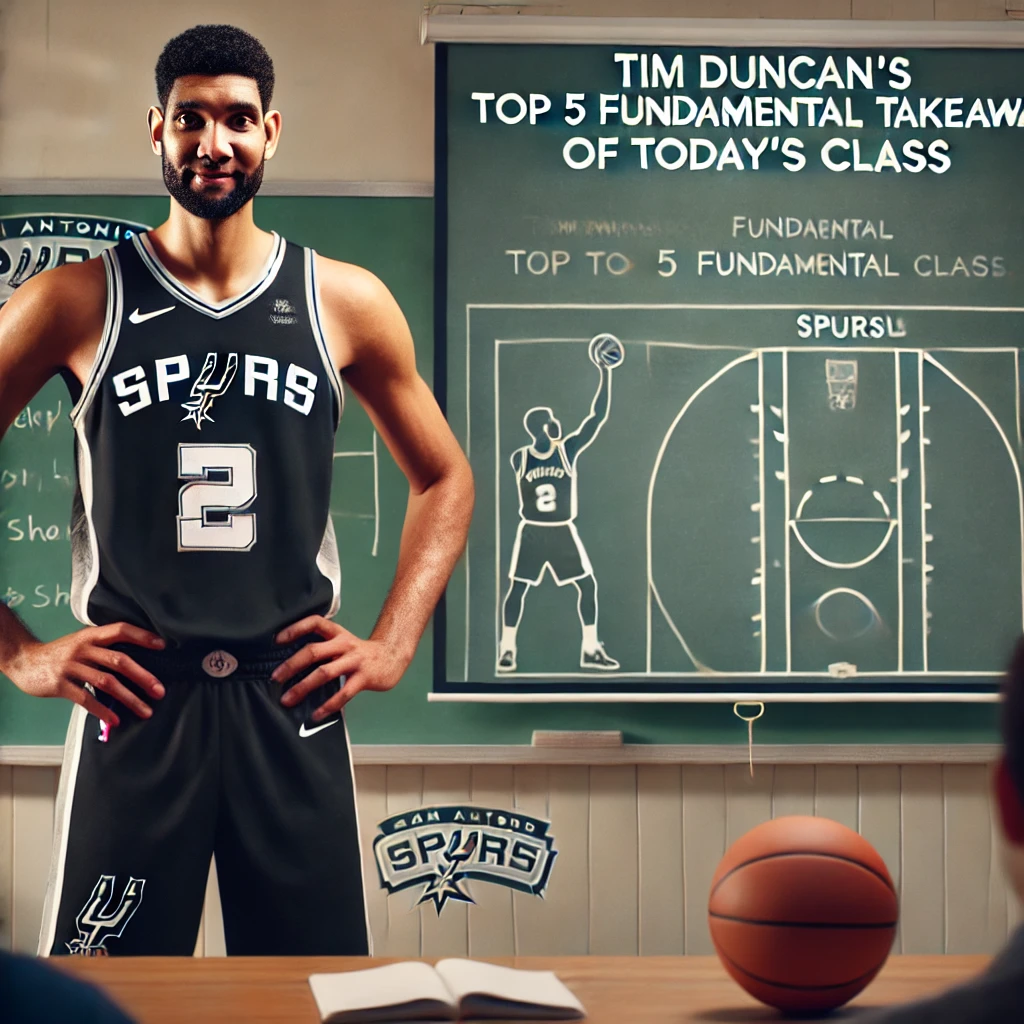
\includegraphics[width=0.75\textwidth]{figures/tim.png}
% \end{frame}
%
% \begin{frame}{Top 5 Fundamental Takeaways}
%     \small
%     \begin{enumerate} \pause
%         \item[5] \textbf{Quicksort is a Divide-and-Conquer Algorithm} – It recursively partitions an array around a pivot and sorts the subarrays efficiently.\pause
%
%         \item[4] \textbf{Partitioning is the Core of Quicksort} – The partitioning step ensures elements are correctly placed around the pivot in $O(n)$ time.\pause
%
%         \item[3] \textbf{Best-case and Worst-case Analysis} – Quicksort runs in $O(n \log n)$ in the best case but can degrade to $O(n^2)$ if poorly partitioned.\pause
%
%         \item[2] \textbf{Randomized Quicksort Helps Avoid Worst-case Behavior} – Choosing a random pivot prevents consistently bad splits and ensures an expected $O(n \log n)$ runtime.\pause
%
%         \item[1] \textbf{Quicksort is Highly Efficient in Practice} – It outperforms merge sort in most cases and benefits from hardware optimizations.
%
%     \end{enumerate}
% \end{frame}

\begin{frame}{Introduction to Algorithms}
    \centering
    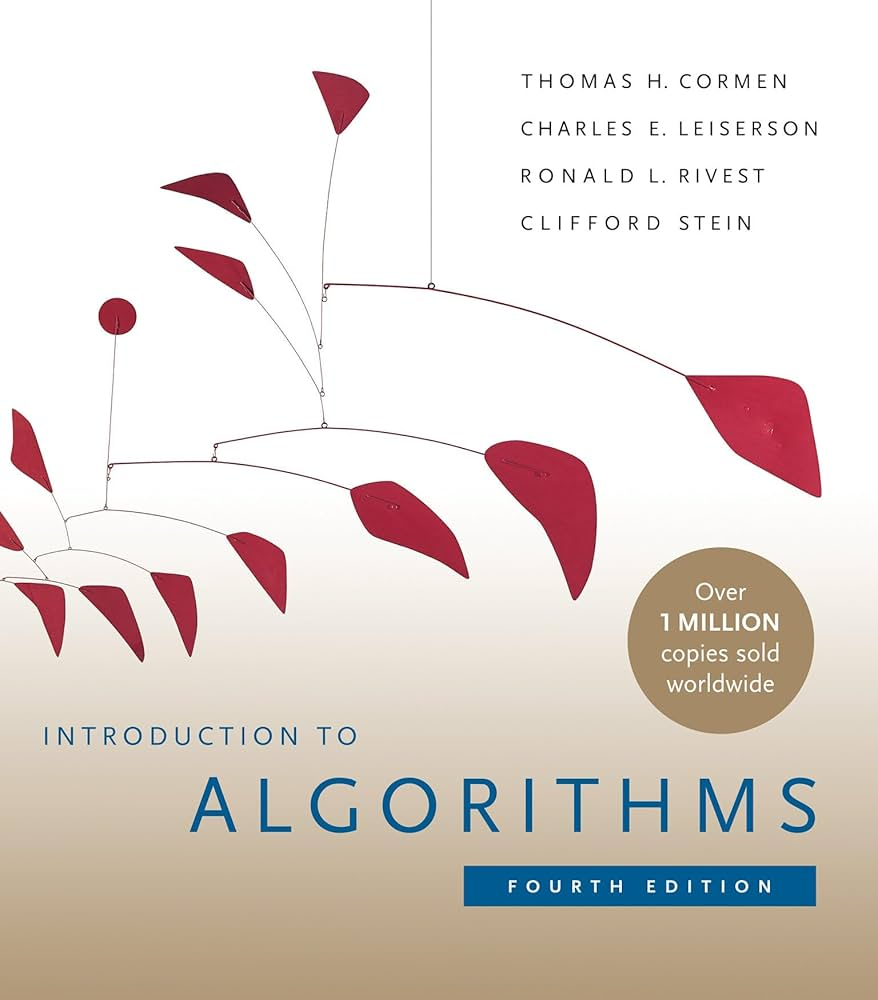
\includegraphics[width=0.45\textwidth]{figures/book_cover.jpg} \\
    \vspace{5mm}{
        \tiny
        Content has been extracted from \textit{Introduction to Algorithms}, Fourth Edition, by Cormen, Leiserson, Rivest, and Stein. MIT Press. 2022.\\
        Visit \url{https://mitpress.mit.edu/9780262046305/introduction-to-algorithms/}.\\
        Original slides from \textit{Introduction to Algorithms 6.046J/18.401J}, Fall 2005 Class by Prof. Charles Leiserson and Prof. Erik Demaine. MIT OpenCourseWare Initiative available at \url{https://ocw.mit.edu/courses/6-046j-introduction-to-algorithms-sma-5503-fall-2005/}.\\
    }
\end{frame}

\end{document}
